% Paquets généraux
\documentclass[a4paper,12pt,titlepage]{article}
\usepackage[T1]{fontenc}
\usepackage[utf8]{inputenc}
\usepackage[french]{babel}
\usepackage[gen]{eurosym}
%\usepackage[dvips]{graphicx}
\usepackage{fancyhdr}
\usepackage{pdfpages} 
\usepackage{multido}
\usepackage{hyperref}
%\usepackage{textcomp}
%\usepackage{aeguill}
\usepackage{schemabloc}
\usepackage[bitstream-charter]{mathdesign}
\usepackage{minted}

\newcommand{\id}{71}
\newcommand{\nom}{Théorie des mécanismes}
\newcommand{\sequence}{04}
\newcommand{\nomsequence}{Liaisons entre les solides}
\newcommand{\num}{02}
\newcommand{\type}{KH}
\newcommand{\descrip}{Liaisons équivalentes, hyperstatisme, liaisons en série et en parallèle, théorie des graphes}
\newcommand{\competences}{B2-12: Proposer une modélisation des liaisons avec leurs caractéristiques géométriques. \\ &  B2-13: Proposer un modèle cinématique paramétré à partir d'un système réel, d'une maquette numérique ou d'u \\ &  B2-17: Simplifier un modèle de mécanisme. \\ &  B2-18: Modifier un modèle pour le rendre isostatique. \\ &  C1-04: Proposer une démarche permettant d'obtenir une loi entrée-sortie géométrique.  \\ &  C2-05: Caractériser le mouvement d'un repère par rapport à un autre repère. \\ &  C2-06: Déterminer les relations entre les grandeurs géométriques ou cinématiques. }
\newcommand{\nbcomp}{7}
\newcommand{\systemes}{}
\newcommand{\systemesnum}{}
\newcommand{\systemessansaccent}{}
\newcommand{\ilot}{2}
\newcommand{\ilotstr}{02}
\newcommand{\dossierilot}{\detokenize{Ilot_02 }}


\newcommand{\auteurun}{Renaud Costadoat}
\newcommand{\auteurdeux}{Françoise Puig}
\newcommand{\institute}{Lycée Dorian}


\usepackage{color}
\usepackage{xcolor}
\usepackage{colortbl}
\usepackage{helvet}
\usepackage[frenchmath]{newtxsf} % for sans serif symbols
\renewcommand{\familydefault}{\sfdefault}
%\usepackage{amsfonts}
%\usepackage{amsmath}
%\usepackage{lmodern}
\usepackage{mathastext}
%\usepackage{xspace}
\usepackage{varioref}
\usepackage{tabularx}
%\usepackage{floatflt}
\usepackage{graphics}
\usepackage{wrapfig}
\usepackage{textcomp}
\usepackage{tikz}
\usepackage{wrapfig}
\usepackage{gensymb}
\usepackage[european]{circuitikz}
\usetikzlibrary{babel}
\usepackage{ifthen}
\usepackage{cancel}
\usepackage{etoolbox}
\usepackage{multirow}
%\usepackage{boxedminipage}
\definecolor{gris25}{gray}{0.75}
\definecolor{bleu}{RGB}{18,33,98}
\definecolor{bleuf}{RGB}{42,94,171}
\definecolor{bleuc}{RGB}{231,239,247}
\definecolor{rougef}{RGB}{185,18,27}
\definecolor{rougec}{RGB}{255,188,204}%255,230,231
\definecolor{vertf}{RGB}{103,126,82}
\definecolor{vertc}{RGB}{220,255,191}
\definecolor{forestgreen}{rgb}{0.13,0.54,0.13}
\definecolor{blcr}{rgb}{0.59,0.69,0.84}
\definecolor{blfr}{rgb}{0.32,0.51,0.75}
\definecolor{orfr}{rgb}{0.90,0.42,0.15}
\definecolor{orcr}{rgb}{0.90,0.65,0.50}
\definecolor{orangef}{rgb}{0.659,0.269,0.072}
\definecolor{orange}{rgb}{0.58,0.35,0.063}
\definecolor{orangec}{rgb}{0.43,0.32,0.25}
\definecolor{rcorrect}{rgb}{0.6,0,0}
\definecolor{sequence}{rgb}{0.75,0.75,0.75}
\definecolor{competences}{rgb}{0.61,0.73,0.35}
\definecolor{grisf}{HTML}{222222}
\definecolor{grisc}{HTML}{636363}
\definecolor{normal}{HTML}{4087c4}
\definecolor{info}{HTML}{5bc0de}
\definecolor{success}{RGB}{92,184,92}
\definecolor{warning}{RGB}{240,173,78}
\definecolor{danger}{RGB}{217,83,79}
\hypersetup{                    % parametrage des hyperliens
    colorlinks=true,                % colorise les liens
    breaklinks=true,                % permet les retours à la ligne pour les liens trop longs
    urlcolor= blfr,                 % couleur des hyperliens
    linkcolor= orange,                % couleur des liens internes aux documents (index, figures, tableaux, equations,...)
    citecolor= forestgreen                % couleur des liens vers les references bibliographiques
    }

% Mise en page
\pagestyle{fancy}

\setlength{\hoffset}{-18pt}

\setlength{\oddsidemargin}{0pt} 	% Marge gauche sur pages impaires
\setlength{\evensidemargin}{0pt} 	% Marge gauche sur pages paires
\setlength{\marginparwidth}{00pt} 	% Largeur de note dans la marge
\setlength{\headwidth}{481pt} 	 	% Largeur de la zone de tête (17cm)
\setlength{\textwidth}{481pt} 	 	% Largeur de la zone de texte (17cm)
\setlength{\voffset}{-18pt} 		% Bon pour DOS
\setlength{\marginparsep}{7pt}	 	% Séparation de la marge
\setlength{\topmargin}{-30pt} 		% Pas de marge en haut
\setlength{\headheight}{35pt} 		% Haut de page
\setlength{\headsep}{20pt} 		% Entre le haut de page et le texte
\setlength{\footskip}{30pt} 		% Bas de page + séparation
\setlength{\textheight}{700pt} 		% Hauteur de l'icone zone de texte (25cm)
\setlength\fboxrule{1 pt}
\renewcommand{\baselinestretch}{1}
\setcounter{tocdepth}{1}
\newcommand{\cadre}[2]
{\fbox{
  \begin{minipage}{#1\linewidth}
   \begin{center}
    #2\\
   \end{center}
  \end{minipage}
 }
}

\newcounter{num_quest} \setcounter{num_quest}{0}
\newcounter{num_rep} \setcounter{num_rep}{0}
\newcounter{num_cor} \setcounter{num_cor}{0}

\newcommand{\question}[1]{\refstepcounter{num_quest}\par
~\ \\ \parbox[t][][t]{0.15\linewidth}{\textbf{Question \arabic{num_quest}}}\parbox[t][][t]{0.93\linewidth}{#1}\par
}


\newcommand{\reponse}[1]
{\refstepcounter{num_rep}
\noindent
\rule{\linewidth}{.5pt}
\textbf{Question \arabic{num_rep}:}
\multido{\i=1+1}{#1}{~\ \\}
}

\newcommand{\cor}
{\refstepcounter{num_cor}
\noindent
\rule{\linewidth}{.5pt}
\textbf{Question \arabic{num_cor}:} \\
}

\newcommand{\titre}[1]
{\begin{center}
\cadre{0.8}{\huge #1} 
\end{center}
}


% En tête et pied de page
\fancypagestyle{normal}{%
  \fancyhf{}
\lhead{\nom}
\rhead{
\includegraphics[width=2cm]{../../img/logo}\hspace{2pt}}
\ifdef{\auteurdeux}{\lfoot{\auteurun,\auteurdeux}}{\lfoot{\auteurun}}
\cfoot{Page \thepage}}

\fancypagestyle{correction}{%
  \fancyhf{}
  \lhead{\colorbox{danger}{\begin{minipage}{0.65\paperwidth} \textcolor{white}{\textbf{Correction}} \end{minipage}} }
  \rhead{
\includegraphics[width=2cm]{../../img/logo}}
  \ifdef{\auteurdeux}{\lfoot{\auteurun,\auteurdeux}}{\lfoot{\auteurun}}
  \rfoot{\colorbox{danger}{\begin{minipage}{0.5\paperwidth} \begin{flushright}\textcolor{white}{\textbf{Correction}}\end{flushright} \end{minipage}} }}

\renewcommand{\footrulewidth}{0.4pt}

\usepackage{eso-pic}
\newcommand{\BackgroundPic}{%
\put(0,0){%
\parbox[b][\paperheight]{\paperwidth}{%
\vfill
\begin{center}
\hspace{0.5cm}\vspace{0.5cm}

\includegraphics[width=\paperwidth,height=\paperheight,%
keepaspectratio]{../../img/fond3}%
\end{center}
\vfill
}}}

\newcommand{\BackgroundPicdeux}{%
\put(25,-30){%
\parbox[b][\paperheight]{\paperwidth}{%
\vfill
\begin{center}

\includegraphics[width=\paperwidth,height=\paperheight,%
keepaspectratio]{../../img/fond4}%
\end{center}
\vfill
}}}

\begin{document}

\pagestyle{empty}

\vspace*{-3\baselineskip}

\AddToShipoutPicture*{\BackgroundPic}

\ifdef{\auteurdeux}{\begin{tabular}{>{\columncolor{gray!00}}m{.3\linewidth} m{.3\linewidth} >{\columncolor{gray!00}}m{.3\linewidth}}
Séquence : \sequence &  \multirow{3}{*}{\hspace{1cm}
\includegraphics[height=1.5cm]{../../img/logo}} &  \begin{flushright} \multirow{4}{*}{\hspace{1cm}\includegraphics[height=4cm]{img/qrcode}}\end{flushright}\\
Document : \type\num \\
 \institute \\
 \auteurun\\
 \auteurdeux
\end{tabular}}{\begin{tabular}{>{\columncolor{gray!00}}m{.3\linewidth} m{.3\linewidth} >{\columncolor{gray!00}}m{.3\linewidth}}
Séquence : \sequence &  \multirow{3}{*}{\hspace{1cm}
\includegraphics[height=1.5cm]{../../img/logo}} &  \begin{flushright} \multirow{4}{*}{\hspace{1cm}\includegraphics[height=4cm]{img/qrcode}}\end{flushright}\\
Document : \type\num \\
 \institute \\
 \auteurun
\end{tabular}}

\vspace{1cm}

\ifdef{\prive}{\begin{center}\colorbox{danger}{\Huge{Avec Correction}}\end{center}}{}

\begin{center}\huge{\nom}\end{center}

\vspace{2cm}

\ifdef{\imagedeux}{\begin{minipage}{0.49\linewidth}}{}
\begin{center}\includegraphics[height=5cm]{/home/renaud/Documents/Renaud/GitHub/django_education/systemes/\imageun}\end{center}
\ifdef{\imagedeux}{\end{minipage}\hfill
\begin{minipage}{0.49\linewidth}
\begin{center}\includegraphics[height=5cm]{/home/renaud/Documents/Renaud/GitHub/django_education/systemes/\imagedeux}\end{center}
\end{minipage}}{}

\vspace{5cm}


\begin{tabular}{p{.15\linewidth} >{\columncolor{white}}p{.8\linewidth}}
    \rowcolor{gray!20}
    Référence & S\sequence\ - \type\num \\
    Compétences & \competences \\
 	\rowcolor{gray!20}
    Description & \descrip \\
    Système & \systemes
  \end{tabular}

\newpage

\AddToShipoutPicture{\BackgroundPicdeux}

\pagestyle{normal}

\section{Activité 1: Détermination de la loi d'entrée/sortie géométrique}

L'objectif de cette partie est de déterminer la loi de fermeture géométrique du système Moby Crea et de la comparer avec celle obtenue par extraction de données expérimentales.

\begin{itemize}
 \item L'angle de rotation du moteur sera appelé $\theta_m$,
 \item La distance AC sera appelée $y$.
\end{itemize}

\begin{center}
 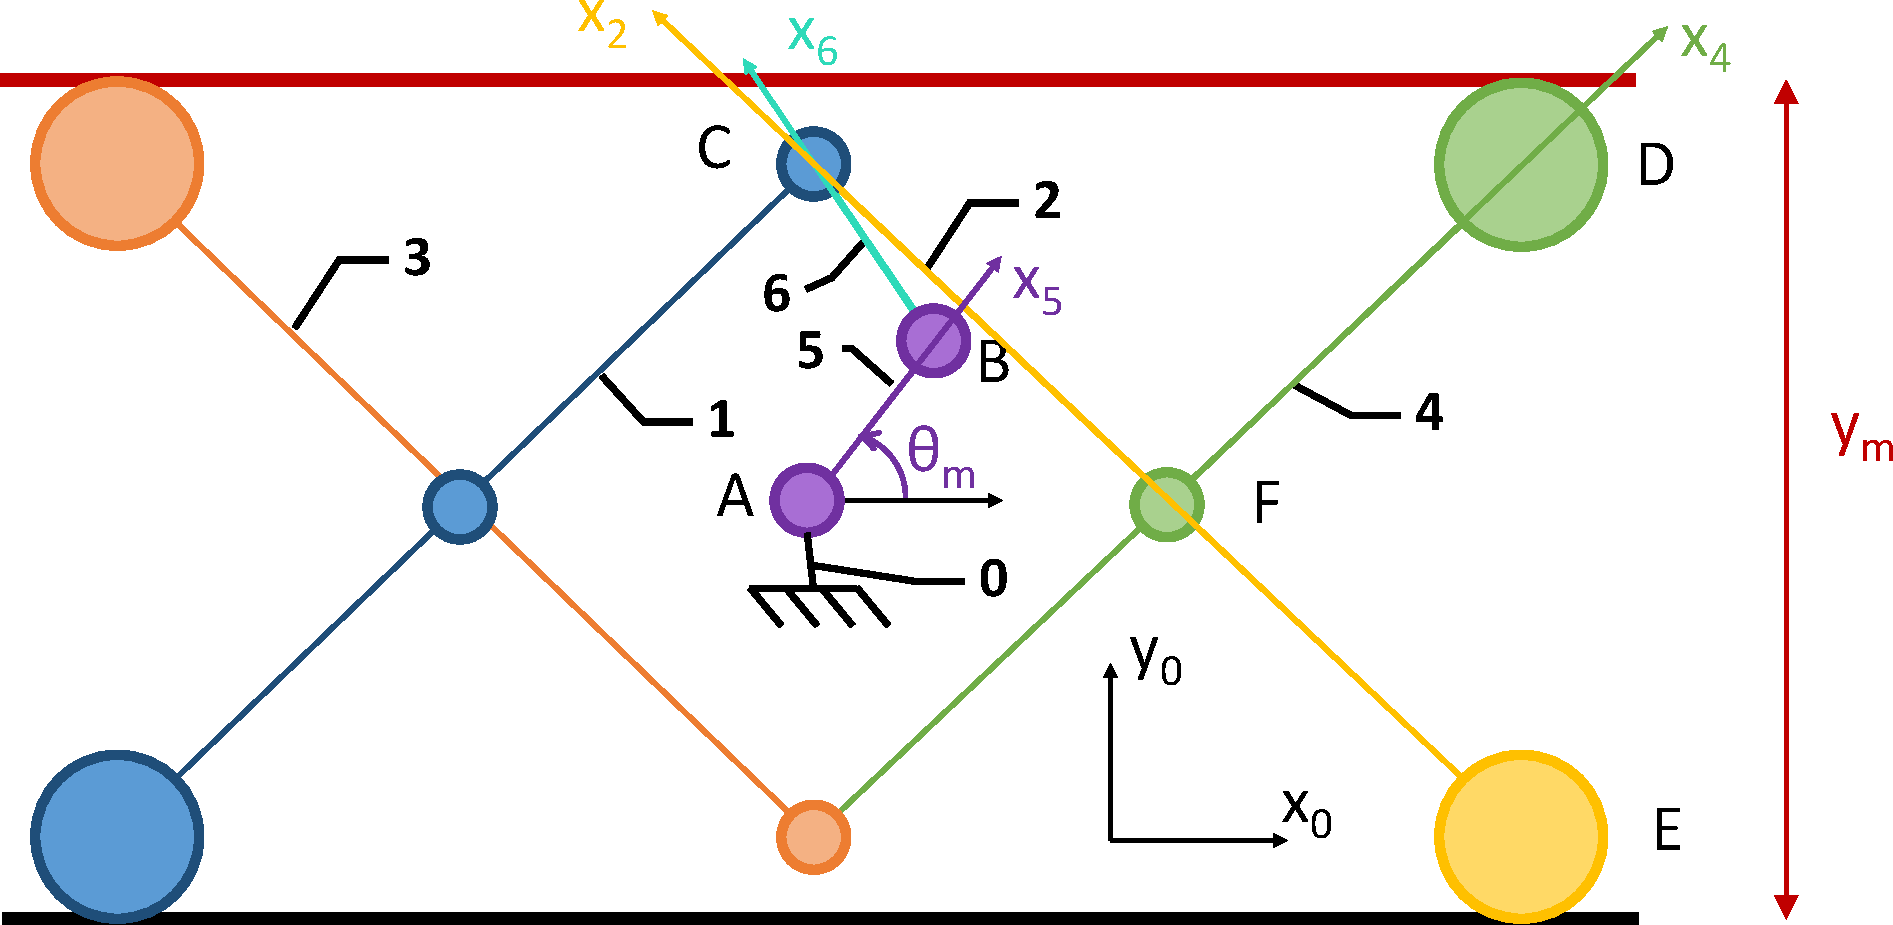
\includegraphics[width=0.6\linewidth]{img/moby_cin}
\end{center}

\paragraph{Question 1:} Déterminer $y$ en fonction de $\theta_m$ et des paramètres géométriques du système, en utilisant la loi de fermeture géométrique. Les dimensions seront mesurées sur le système afin d'effectuer l'application numérique.

\paragraph{Question 2:} Sur le logiciel \textit{Scilab}, faire varier $\theta_m$ de $0$ à $6\pi$ (\texttt{a=(0:0.1:6*\%pi)}).

Puis calculer les valeurs de $y$ (\texttt{t=f(a)}).

Enfin demander au logiciel de tracer la fonction $t=f(a)$ (\texttt{plot2d(a,t)}).
%
%\paragraph{Question 3:} Après avoir récupéré le résultat d'une simulation sur le logiciel du Moby Crea traçant la vitesse de rotation du bras en fonction de celle du moteur. Importer ces résultats sur le logiciel Scilab et intégrer numériquement ces courbes, vous proposerez un algorithme afin d'effectuer cette intégrale.
%
%L'importation est possible si le fichier a été mis sous la forme:
%\begin{center}
%\texttt{0.000  0.000} \\
%\texttt{0.063  0.063} \\
%\texttt{0.127  0.127} \\
%\texttt{0.190  0.189} \\
%\texttt{0.254  0.251}
%\end{center}
%
%La commande \texttt{[x]=read (fichier ,m ,n [, format])} permet d'intégrer les données sous la forme d'une matrice.
%
%\begin{itemize}
% \item \texttt{fichier} : Chaîne de caractère correspondant au nom du fichier,
% \item \texttt{x} : matrice, vecteur ou chaîne de caractères,
% \item \texttt{m} : entier, nombre de ligne à lire, m=-1 permet de lire toutes les lignes du fichier,
% \item \texttt{n} : entier, nombre de colonnes à lire,
% \item \texttt{format} : chaîne de caractère au format Fortran (ne pas utiliser).
%\end{itemize}
%
%\paragraph{Question 4:} En utilisant le résultat de l'intégrale de la vitesse de rotation du moteur comme donnée d'entrée, calculer les valeurs de $\theta$ (\texttt{t=f(a)}) et les comparer à celles obtenues numériquement.

\section{Activité 2: Détermination de la loi d'entrée/sortie cinématique}

Cette partie permettra de déterminer la loi d'entrée à imposer au moteur électrique afin de permettre d'obtenir un déplacement souhaité du bras.

\begin{itemize}
 \item La vitesse de rotation du moteur sera appelée $\omega_m=\dot{\theta_m}$,
 \item La vitesse de rotation du bras sera appelée $v=\dot{y}$.
\end{itemize}

\paragraph{Question 1:} Déterminer $\omega_m$ en fonction de $v$ et des paramètres géométriques du système, en utilisant la loi de fermeture cinématique. Les dimensions seront mesurées sur le système afin d'effectuer l'application numérique.

%\subsubsection{Trapèze de vitesse}
%
%L'objectif est d'obtenir le profil suivant pour la vitesse de rotation du bras par rapport au bâti.
%
%\begin{center}
% 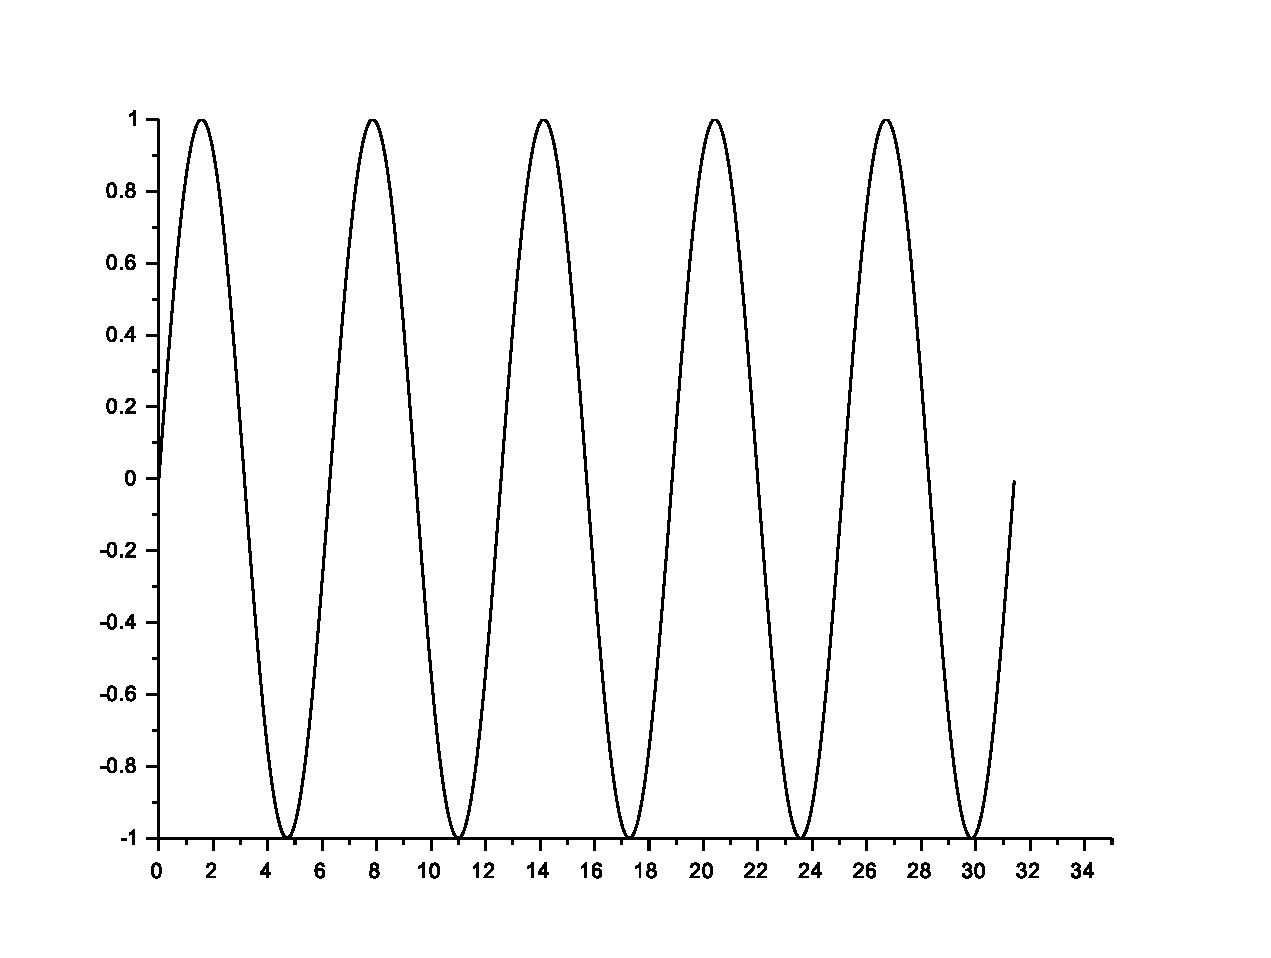
\includegraphics[width=0.6\linewidth]{img/moby_profil}
%\end{center}
%
%\paragraph{Question 2:} En déduire le profil de vitesse à imposer au moteur $\omega_m$. Vous tracerez ce profil en utilisant les commandes suivantes.
%
%\begin{itemize}
% \item Temps total de montée $1s$: \texttt{t1=(0:0.1:1)},
% \item Temps total de maintient $2s$: \texttt{t2},
% \item Temps total de descente $1s$: \texttt{t3},
% \item Montée constante jusqu'à $0.15rad.s^{-1}$: \texttt{v1=k*t1+k0},
% \item Maintient à $0.15rad.s^{-1}$: \texttt{v2},
% \item Descente jusqu'à $0rad.s^{-1}$: \texttt{v3},
% \item temps total $t$: \texttt{t=[t1 t2 t3]},
% \item Profil complet de $\omega_b$: \texttt{ob=[v1 v2 v3]},
% \item Tracé du profil de $\omega_b$: \texttt{plot2d=(t,ob)},
% \item Calcul de $\omega_m$: \texttt{om=f(ob)},
% \item Tracé du profil de $\omega_m$: \texttt{plot2d=(t,om)}.
%\end{itemize}
%
%Ce profil de vitesse devra être utilisé comme loi d'entrée pour le modèle Soldiworks élaboré lors de l'activité 3.

\section{Activité 3: Modélisation sur un modeleur 3D}

Le logiciel Solidworks va permettre de déterminer les lois d'entrée sortie géométrique et cinématique du système Moby Crea.

Le fichier à ouvrir pour cette étude est le fichier \verb?SW/_Moby-Crea.SLDASM?.

\begin{itemize}
 \item La vitesse de rotation du moteur sera appelée $\omega_m=\dot{\theta_m}$,
 \item La vitesse de rotation du bras sera appelée $v=\dot{y}$.
\end{itemize}

\paragraph{Question 1:} Sur Solidworks, paramétrer le Moby Crea sur le logiciel Meca3d afin de pouvoir simuler son comportement.
 
\begin{itemize}
 \item Tracer $y=f(\theta_m)$,
 \item Tracer $v=f(t)$,
\end{itemize}

%\paragraph{Question 2:} Construire une courbe de la forme du profil de vitesse en trapèze.
%
%Avec:
%\begin{itemize}
% \item $t_1=1s$,
% \item $t_2=3s$,
% \item $t_{total}=5s$,
% \item ${\omega_b}_{max}=0.15rad.s^{-1}$.
%\end{itemize}
%
%\paragraph{Question 3:} Utiliser cette courbe comme donnée d'entrée pour calculer la vitesse $\omega_m$ en fonction du temps. Comparer ce résultat avec celui de l'activité 2.
%
%\paragraph{Question 4:} Construire une courprofbe à partir de la fonction $\omega_m$ calculée lors de l'activité 2. Montrer que cela revient exactement au tracé précédent.

\section{Activité 4: Système acausal}

Cette partie va permettre d'introduire le modèle \og acausal \fg afin de déterminer si celui qui a été mis en place pour le Moby Crea en est un. Un modèle \og acausal \fg est un modèle qui ne possède pas de lien cause à effet. Il revient à des équations implicites sans ordre entre les variables et sans spécification d'entrée et de sortie.

\paragraph{Question 1:} A la vue de la définition précédente, pensez-vous que ce système puisse être modélisé par un modèle \og acausal \fg ?

\paragraph{Question 2:} Vous effectuerez la liaison entre les activités afin de récupérer les résultats de l'activité 2 pour les utiliser sur Solidworks durant l'activité 3.

\paragraph{Question 3:} Vous montrerez l'influence sur les résultat des dimensions géométriques du système afin de déterminer si leur choix dépend des données cinématiques.

\end{document}

\pagestyle{correction}\setcounter{section}{0}

\paragraph{Question 1:}
\end{document}